Figure~\ref{fig:4:fw} in Chapter~\ref{chap:cc.fw} shows the structure of the
congestion control framework described in this thesis. The framework
categorizes \emph{In-path} and \emph{Out-of-path} sources and
\emph{out-of-band} signaling for implementing congestion control, which are
discussed in this chapter. This chapter is based on our work on congestion
control for interactive multimedia applications, which is documented in
\citepub{c:3grc} and \citepub{c:glass}.

In a 3G network, mobility, cell loading, handovers and other factors can
affect the throughput available to each user and the varying network capacity
affects the video quality~\cite{diaz2007evaluating}. Deployments of GPRS, 3G
and LTE show that there are still geographical areas where capacity is
constrained~\cite{Curcio:glass, 6576402}. These constrained geographical areas
may occur due to fading and interference from large building structures or
closed or inaccessible areas (e.g., tunnels, boats on lakes or in the
archipelago, rural areas).

In \citepub{c:3grc}, when the available link capacity changes at a base
station, it notifies the endpoint connected to it about the current capacity.
Based on the notifications the sender adapts the media sending rate. Hence,
this paper covers the \emph{in-path} sources and \emph{out-of-band} signaling
of the framework defined in Chapter~\ref{chap:cc.fw}.

In \citepub{c:glass}, we explore the use of coverage maps for congestion
control. The map server collect throughput information from the mobile
clients, which also add geo-location information along with the throughput
information. This assists the map server to build a bandwidth and coverage map
and is queried by the mobile to predict coverage outage. This paper covers the
\emph{out-of-path} sources (e.g., coverage map) signaling congestion cues
\emph{out-of-band} to the endpoints.

\section{In-path Congestion Cues}

% ECN, PCN, BW indication

In some network deployments, routers along the media path are capable of
detecting congestion before the queue overflows, typically, using active queue
management (e.g., RED). A router marks a packet, indicating that the packet
experienced congestion and the router would soon drop packets for this
flow~\cite{rfc3168}. The receiver on receiving this indication keeps a counter
for the number of ECN marked IP packets and signals it to the sender. For
performing congestion control, the sender typically treats the count of ECN
marked packets as lost packets~\cite{rfc6679}. For example, the sender uses
the sum of the reported loss events and the reported ECN events as the
\emph{p} (loss) value in the TFRC equation. Network-Assisted Dynamic
Adaptation (NADA)~\cite{rmcat-nada} propose a delay-based congestion control,
the receiver measures congestion by aggregating the packet loss count,
reported ECN markings, and one-way delay measurements into a single cue. The
sender calculates the new rate based on the variation in the delay cue
compared to earlier measurements and the priority of the multimedia
stream~\cite{pv-nada}.

\begin{figure}
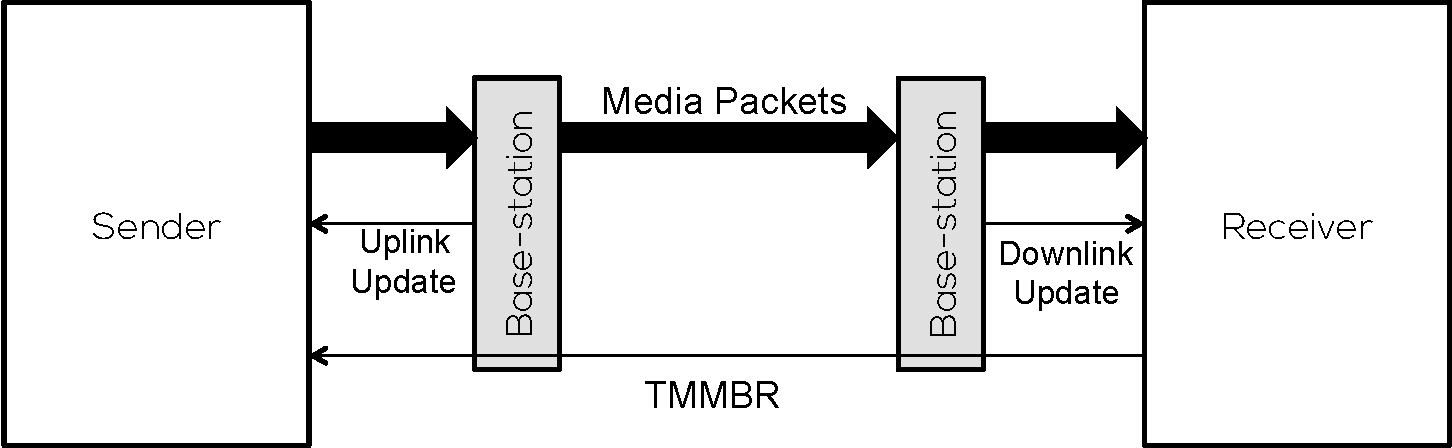
\includegraphics[width=\textwidth]{chap8-fig-tmmbr}
\caption{Endpoints receiving capacity indication from the middleboxes for implementing congestion control.}
\label{fig:cc:tmmbrab}
\end{figure}

In wireless networks, such as 3G/LTE, the last hop is typically the bottleneck
because the core network is well provisioned. In \citepub{c:3grc}, we
implement a network-assisted congestion control scheme, wherein, base-stations
(along the media path) notify the mobile terminals about the available link
capacity. In TMMBR-A, the base-stations notify both the sending and receiving
endpoints about the available capacity, i.e., the sender is notified about the
uplink capacity and the receiver is notified about the downlink capacity. If
an endpoint sends and receives data, it is notified asynchronously about the
uplink and downlink capacity. In TMMBR-B, only the receiving endpoint is
notified about the downlink capacity. Both TMMBR-A and TMMBR-B employ a
co-operative congestion control scheme, wherein the receiver sends a TMMBR
request to the sender containing the current downlink capacity. In TMMBR-A the
sender also receives a notification about the uplink capacity from the
base-station, hence, comparing the request from the receiver and the
notification from the base-station, it chooses the minimum of the two values
as the new sending rate. In TMMBR-B, the sender implements calculates the
\emph{sender's estimate} (similar to the one described in~\ref{cc:co-op}) and
chooses the minimum of the sender's estimate and the receiver's bit rate
request. Figure~\ref{fig:tmmbn} shows the performance of TMMBR-A and TMMBR-B,
where both endpoints are sending media over a 3G network.

\begin{figure}
  \centerline{
    \subfloat[TMMBR-A]{
      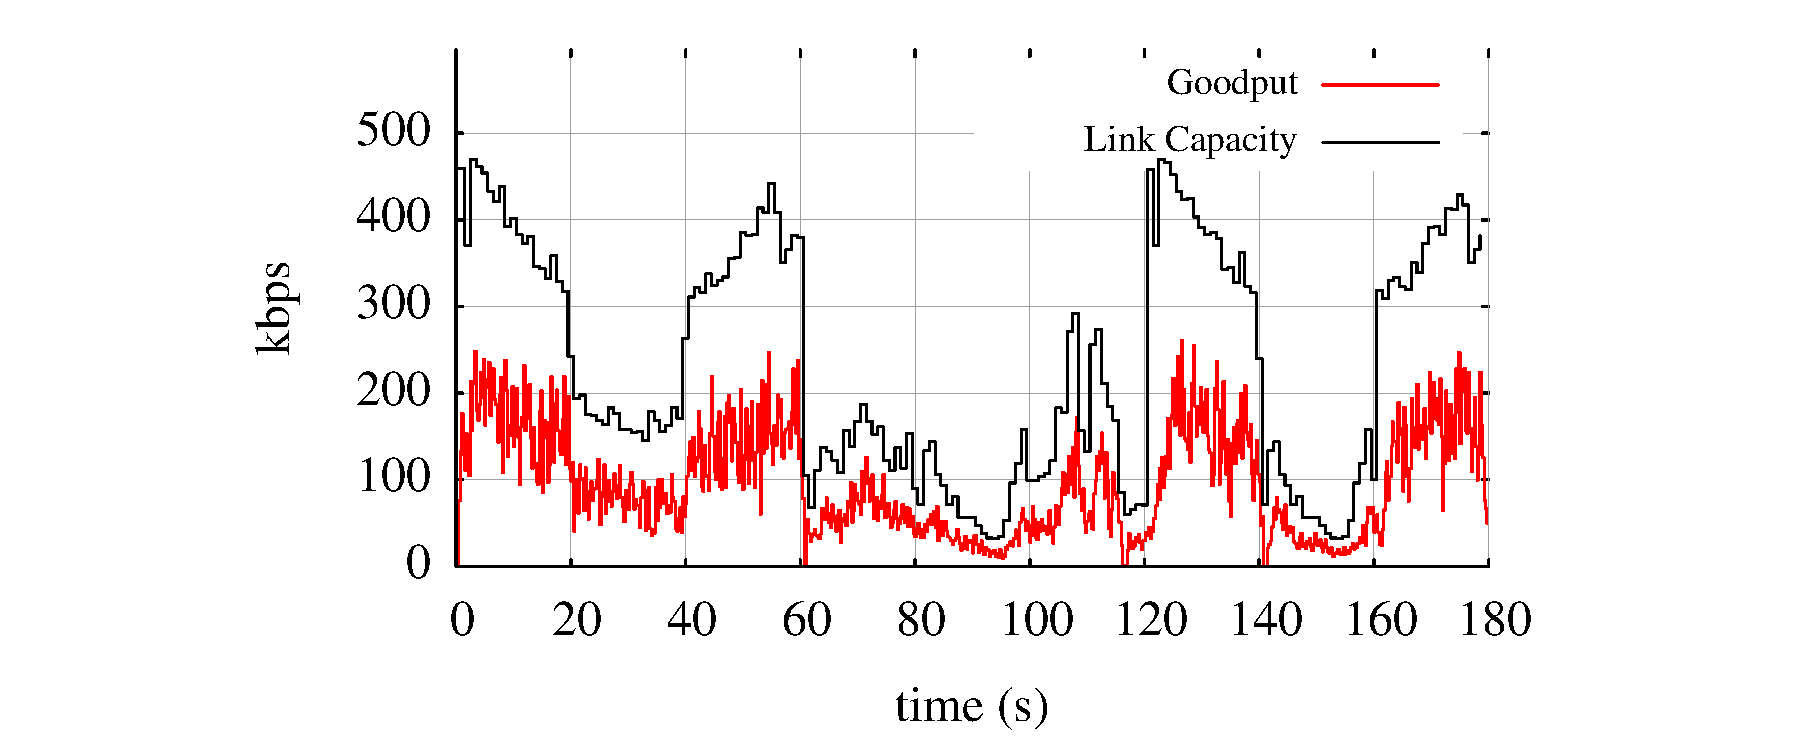
\includegraphics[width=0.5\textwidth, clip=true, trim=3cm 0 4.5cm 0]
      {chap8_graph_3g_tmmbr_a}
    }
    \subfloat[TMMBR-B]{
      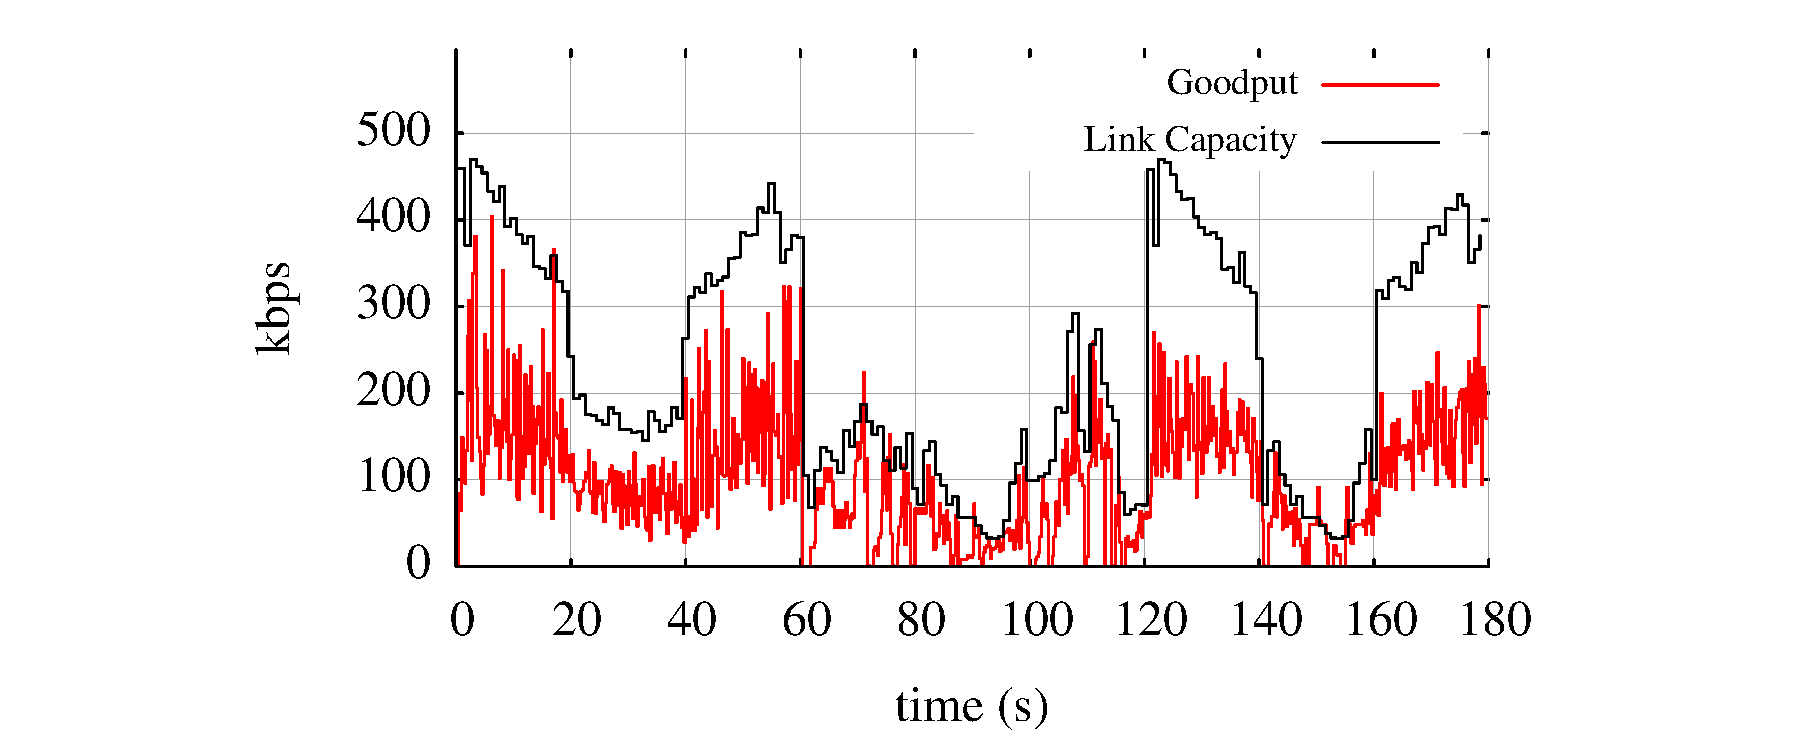
\includegraphics[width=0.5\textwidth, clip=true, trim=3cm 0 4.5cm 0]
      {chap8_graph_3g_tmmbr_b}
    }
  }
  \caption{Performance of bandwidth indications by the base stations a)
  TMMBR-A: both terminals are assisted, b) TMMBR-B: only receiver is
  assisted.}
  \label{fig:tmmbn}
\end{figure}


\section{Out-of-path Congestion Cues}

% Congestion map

Service Maps are presented in~\cite{1630563} and the measurement based
approach is proposed in~\cite{Aravinda:2008p14}. GPS-based congestion control
is introduced in~\cite{Yao:2008p21}, and evaluated in different
scenarios~\cite{Yao:2009p57}, \cite{Yao:2010p64}, but they take signal
strength as an influential factor for rate-control and show that predicting
based on signal strength alone is insufficient. Yet, their results indicate
that past information can be used to predict future network characteristics.

To overcome these challenges, in \citepub{c:glass}, we implement a bandwidth
coverage map that collects connectivity information from the users
(\emph{crowd-sourcing}) and calculates the available capacity at the reported
geographical locations. \cite{6012045} also proposes a similar architecture
(\emph{bandwidth lookup service}) to the one in \citepub{c:glass} and uses
different types of averaging algorithms to predict future network
characteristics in Dynamic Adaptive Streaming over HTTP (DASH). While the
averaging algorithm is not a focus of this thesis, we use
K-means~\cite{Kanungo:2002:LSA:513400.513402} and K-nearest neighbor
(K-NN)~\cite{Iwerks:2003:CKN:1315451.1315496} algorithms to form regions with
similar bandwidth. Details of the averaging algorithms can be read
in~\cite{sharmistha-thesis}. Additionally, \cite{Riiser:2012:2240136} proposes
fetching the bandwidth along a travel route in steps of 100 meters, which we
find limiting. Instead we propose multiple methods for discovering areas with
poor connectivity and show that not only looking up future bandwidth but also
when to vary the sending rate (\emph{prefetch}) affects the usefulness of the
service. A preliminary analysis using simulations of our system is done
in~\cite{Curcio:glass}.

\begin{figure}
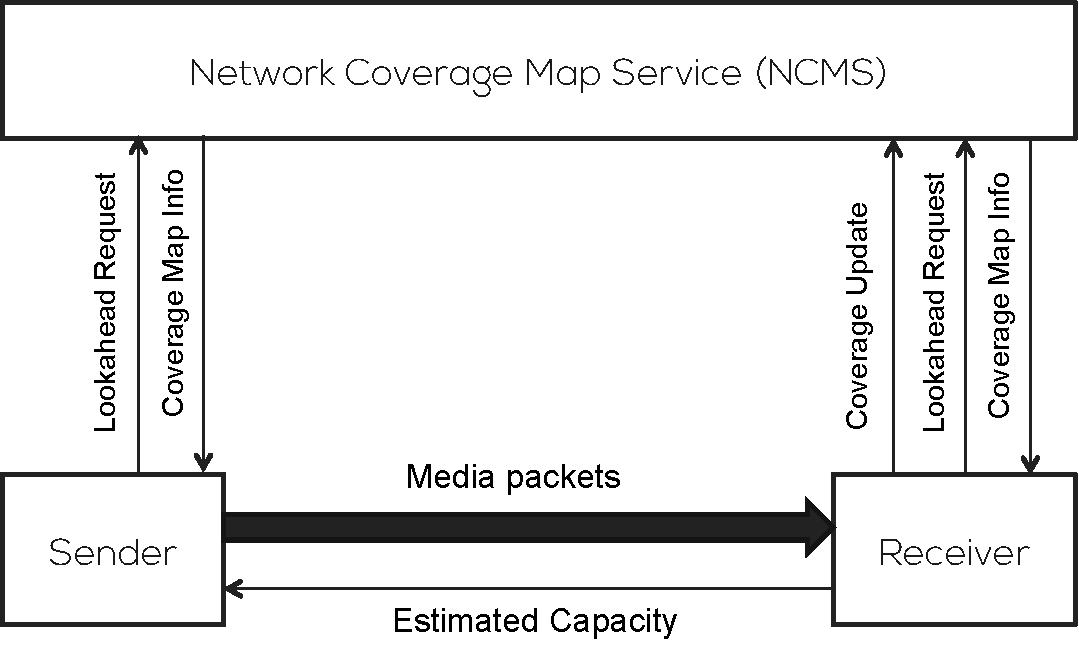
\includegraphics[width=\textwidth]{chap8-fig-ecv}
\caption{Endpoints using a Network Coverage Map Service to send coverage updates, query for upcoming congestion and receive coverage updates.}
\label{fig:cc:ecv}
\end{figure}


In \citepub{c:glass}, we presented a mechanism enabling an endpoint (usually a
receiver) to proactively react to upcoming capacity limitations in wireless
access networks. The receiver uses hints provided by a network coverage map
service (NCMS), which uses crowd sourcing to gather the coverage and capacity
information. These hints are sent to the sender, which can alter the sending
rate. We find that the information provided by the NCMS is suitable for both
predictive rate-switching and pre-buffering and helped in avoiding almost all
packet losses in the scenarios we investigated, noticeably increasing video
quality. While these results are promising, they are only a first step: flash
crowd effects resulting from many clients approaching and/or creating a
coverage hole at the same time require further study. Similarly, the
performance impact for a more encompassing geographical coverage and more
diverse network connectivity deserves further investigation.
